\section{Introduction}
A long-term goal of robotics research is the introduction of intelligent household robots.
To be effective, such robots will need to perform complex tasks
over long horizons (e.g., setting a dinner table, doing laundry). Planning for these long-horizon tasks is infeasible
for state-of-the-art motion planners, making the need
for a hierarchical system of reasoning apparent.

One way to approach hierarchical planning is through combined \emph{task and motion planning} (TAMP). In this
approach, an agent is given a symbolic, logical characterization of actions (e.g., move, grasp,
putdown), along with a geometric encoding of the environment. TAMP systems maintain a hierarchical
separation of high-level, symbolic task planning and low-level, geometric motion planning.
Efficient integration of these two types of reasoning is difficult, and recent research has
proposed several methods for it~\cite{srivastava2014combined, kaelbling2011hierarchical,
lagriffoul2014orientation, GarrettWAFR14, dornhege2012semantic}.

\begin{figure}[t]
  \centering
    \noindent
    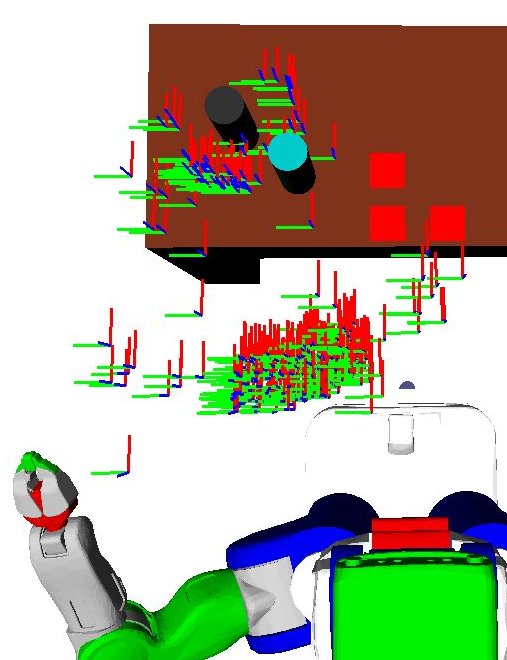
\includegraphics[scale=0.15]{images/move_grasp.png}\hspace{5 mm}
    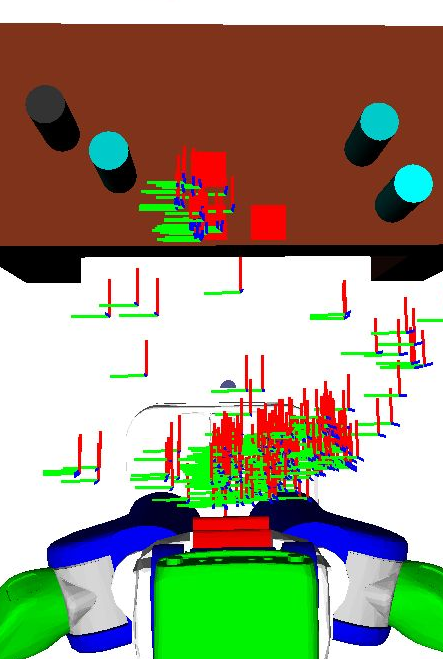
\includegraphics[scale=0.15]{images/move_putdown.png}
  \caption{\small{Screenshots showing distributions learned by our system in a simulated pick-and-place
    domain. We use reinforcement learning to train good sampling distributions for continuous motion
    planning parameters in long-horizon tasks. The robot must grasp the black can and put it down
    on the red square. The left image shows learned base position (blue) and grasping (green) distributions,
    and the right shows learned base position (blue) and putdown (green) distributions. The grasping policy
    learned to avoid the obstructions.}}
  \label{fig:cover}
  \vspace{-1.5 em}
\end{figure}

We adopt the principles of abstraction developed by Srivastava et
al.~\cite{srivastava2014combined} (henceforth referred to as SFRCRA-14) to factor the required reasoning and
search problems into interacting logic-based and geometric components. In this approach, the
logic-based layer of abstraction is refined with additional information gained from geometric reasoning.

SFRCRA-14 uses a (classical) task planner to produce a symbolic plan containing
a sequence of actions to reach a goal state. Then, in a process known as \emph{plan refinement},
candidate values are proposed for the continuous variables in this symbolic plan.
These values are checked locally for feasibility by calling a motion planner.
The system conducts a greedy search to find a symbolic plan for which
a motion planning feasible refinement is possible. Although this algorithm achieves good results
in a class of domains, it is complete only in some situations; in
general, it may not find solutions to solvable problems.

The TAMP paradigms referenced above all use hand-coded
heuristics to instantiate symbols with continuous values.
The search for instantiations of symbolic
references typically uses domain-specific insight from the user to reduce
the space of possible values. For example, in SFRCRA-14,
end effector grasp poses for a can in a pick-and-place task are sampled around the can in
each of the 8 cardinal and intermediate directions, at a fixed
distance and height. Such coarse distributions require
fine-tuning for each domain and lack robustness to increased
environmental complexity.

We introduce a complete algorithm for TAMP that daisy-chains plan refinement (the search for symbolic
reference instantiations) with the search for which symbolic plan to try refining, given options that address different
infeasibilities. Furthermore, we present machine learning techniques to train heuristic
functions that guide both of these search processes.

Reinforcement learning (RL) refers to the process of an agent learning a policy (a mapping from states to actions)
in its environment that maximizes rewards. Zhang and Dietterich~\cite{JobShopSched} first applied the RL framework
to planning problems, using a job shop scheduling setting. In this work, we take inspiration from
their approach; we use RL to train continuous proposal distributions for
plan refinement, thus avoiding the discretization common to TAMP systems. We implement our approach using methods adapted from
Zucker et al.~\cite{workspacebias}, who train a configuration space sampler for motion planning
using features of the discretized workspace.

The five contributions of our work are as follows: 1) we present a complete algorithm for TAMP
by maintaining a \emph{plan refinement graph} to select which symbolic plan to try refining;
2) we present randomized refinement, a local search
algorithm for plan refinement that is easily formulated as an MDP; 3) we formulate plan refinement in the
RL framework and learn a policy for this MDP; 4) we train heuristics to search intelligently
through a plan refinement graph; and 5) we present experiments to evaluate our approach in a variety of simulated
domains. Our results demonstrate that our approach yields significantly improved
performance over that of SFRCRA-14.
